\section*{Detekce světelných stop v obraze}
Pro analýzu vlastností broušeného kamene je důležité detekovat světelné stopy vzniklé dopadem laserový svazků, vystupujících z kamene umístěného v naší experimentální soustavě, na stínítko. Zároveň je třeba určit parametry stop, které je možné porovnat s parametry svazků matematického modelu kamene v LADOKu. 

Pří zkoumání obrazu, lze intenzity pixelu rozložit na dvě základní složky. Mezi ně patří velikost pozadí a příspěvek od odpadajícího laserového svazku. Ve zjednodušeném případě lze říci, že po odečtení pozadí získáme oblasti, kde se nachází laserové stopy. Při detekci laserových stop však narážíme na řadu problémů.

Prvním problémem je určení samotného pozadí. Jednoduchou myšlenkou by bylo prahování obrazu nad konstantní úrovní. V našem obraze však pozadí typicky konstantní není. Po dopadu laserového svazku na drsné stínítko se nezanedbatelná část záření difuzně odrazí. Odrazivé vlastnosti materiálu závisí na úhlu odpadajícího světla a lze je matematicky popsat pomocí abstrakce zvané BRDF (Bidirectional reflectance distribution function). BRDF se navíc může v různých částech stínítka lišit z důvodu rozdílné koncentrace příměsí v materiálu. Odrazivost materiálu zapříčiní nárůst intenzity světla nejen v místě dopadu světelného svazku, ale i v jeho okolí. Nejznatelnější nárůst intenzity záření pozorujeme v blízkém okolí stopy. Z toho důvodu je třeba počítat s dynamicky měnící se hodnotou pozadí, která závisí především na zářivém toku, hustotě a úhlu dopadajících svazků. Rozdílné pozadí se může také vytvořit odrazem zdrojového svazku od jiných předmětů, než broušeného kamene. Hlavním příspěvkem je v tomto případě odraz od podstavce, na který pokládáme broušený kámen.

Další nepříjemnost nastává při překrývání laserových stop. Odfiltrováním pozadí získáme oblasti, kde se nachází světelné stopy. Pokud dochází k překrytí dvou či více stop nevystačíme pouze s jednoúrovňovým prahováním \cite{Drapela}, ale oblasti je třeba rozčlenit pomocí víceúrovňového prahování. V místě, kde je vysoká koncentrace svazků mohou dokonce svazky dopadnout tak blízko sebe, že splynou v jednu stopu (obr. \ref{Splynuti}). Zároveň předpokládáme, že se laserové stopy nepřekrývají příliš často abychom byli schopni určit pozadí.   

\begin{figure}[htbp]
    \centering
    \begin{minipage}[c]{0.48\textwidth}
        \centering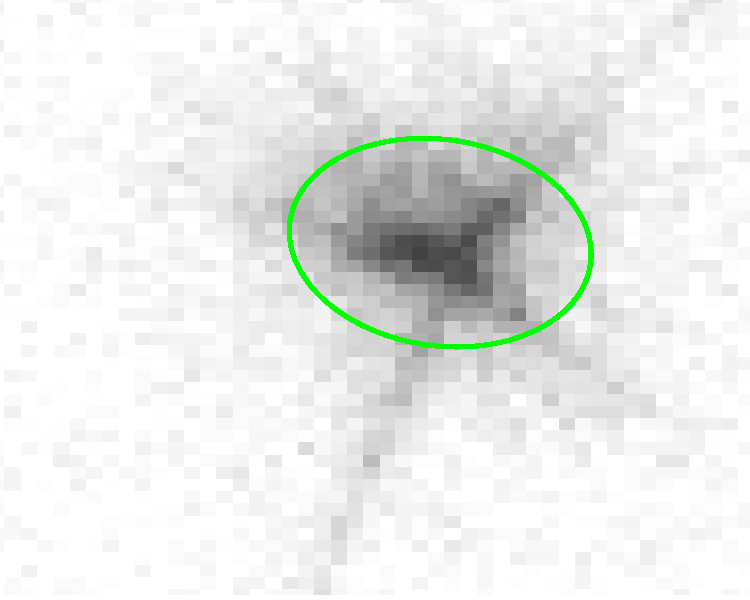
\includegraphics[width=.6\textwidth]{pf_near.pdf}
    \end{minipage}
    \begin{minipage}[c]{0.48\textwidth}
        \centering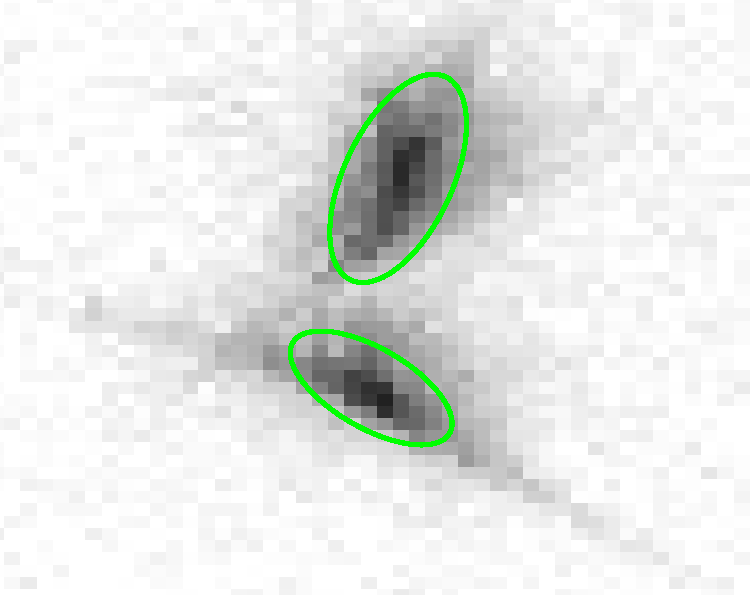
\includegraphics[width=.6\textwidth]{pf_near2.pdf}
    \end{minipage}
    \\
        \caption[Slynutí dvou různých svazků.]{Ilustrace slynutí dvou různých svazků. V pravém i levém snímku se nachází typově stejné laserové svazky. Na levém obrázku dopadly na stínítko příliš blízko sebe. V tomto případě detekujeme pouze jednu stopu.}
        \label{Splynuti}
\end{figure}

Detekci zároveň komplikuje všudepřítomný šum a obraz je třeba filtrovat. Filtrováním snížíme šum v odraze, ale zároveň zmenšíme kontrast mezi stopami. 

Ne všechny svazky vystupující z kamene je možné detekovat. Svazky s vícenásobným odrazem postupně ztrácí zářivý tok. Po dopadu na stínítko mohou splynout se šumem a jejich detekce je prakticky nemožná. Mezi stopami s nízkým jasem se zároveň často objevují artefakty vzniklé nežádoucími optickými efekty např. interferencí, proto detekce bude často selhávat, pokud chceme rozpoznat i nepatrné stopy v obraze.



%%tohle bych zařadil na později
%Laserové stopy chceme detekovat v černobílém HDR snímku půlkulového stínítka, na které dopadá část laserových svazků vystupujících z nasvíceného kamene. Snímek ze zatížen radiálním zkreslením, které je způsobeno vlastností optické soustavy objektivu. Radiální zkreslení bylo určeno v předchozí bakalářské práci \cite{Drapela}. Snímek lze pomocí transformace z \cite{Drapela} zkreslení zbavit. Z \cite{Drapela} navíc známe transformaci mezi pozicí bodu v nezkresleného snímku a odpovídajícím parametrům azimutu a elevace.

\begin{figure}[htbp]
    \centering
    \begin{minipage}[c]{0.48\textwidth}
        \centering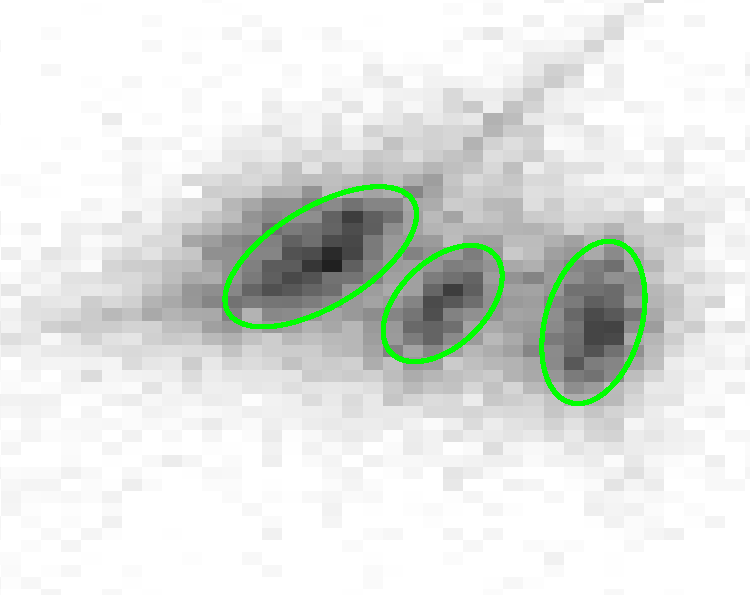
\includegraphics[width=.7\textwidth]{pf_punch2.pdf}
    \end{minipage}
    \begin{minipage}[c]{0.48\textwidth}
        \centering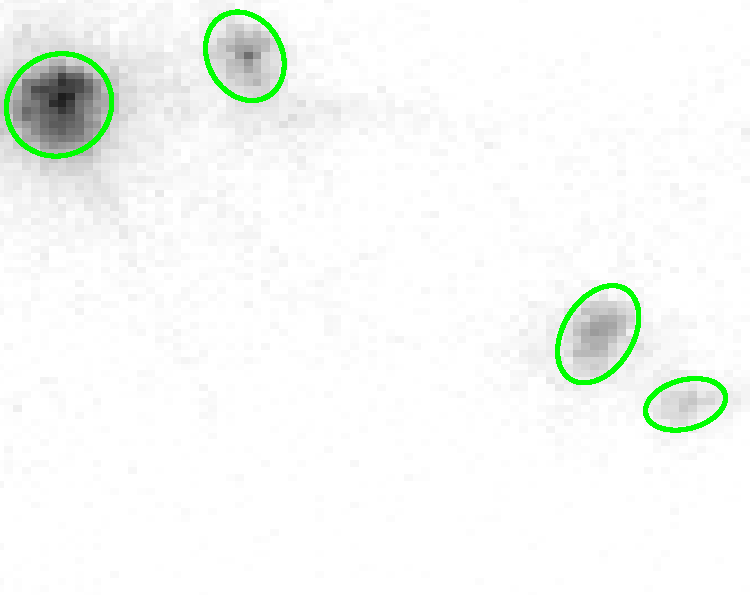
\includegraphics[width=.7\textwidth]{pf_deff2.pdf}
    \end{minipage}
    \\
        \caption[Problémové detekce.]{Problémové detekce. Nalevo jsou laserové stopy blízko u sebe. Stopy je nutné od sebe oddělit. Na levém snímku jsou znázorněny markantní rozdíly mezi velikostí a intenzitou stop. Je nutné použít víceúrovňový detektor. }
        \label{Detekce}
\end{figure}

\section*{Předchozí práce}

V předchozí práci \cite{Drapela} se využívalo odfiltrování pozadí obrazu a následné jednoúrovňové prahování podle intenzity. Tento přístup však nedetekoval stopy s menší intenzitou než nastavený práh a laserové stopy umístěné blízko u sebe spojil do jedné. 

Bohatší pojetí problému se objevilo v Bodlákově práci \cite{Bodlak2005}. Snímek se prahoval více než jedním prahem, přičemž z oblastí nad prahem se sestavila stromová struktura a světelné stop se určily jako listy stromu s dostatečnou významností. Tento přístup je však pro svou výpočetní náročnost nepoužitelný pro snímky s rozlišením \textit{2050x2050}, které máme k dispozici. 

Naše úloha detekce je velmi podobná detekci hvězd a galaxií v astronomických snímcích. V oblasti astronomie se hojně používá program s názvem Source Extractor \cite{SEXarticle}. Tento program má za sebou dlouholetý vývoj, je optimalizován z hlediska rychlosti a odzkoušený širokou veřejností. Tento software lze po naladění parametrů použít i pro náš případ. Nevýhodou však je, že nelze spustit operačním systémem Windows, který využíváme a neposkytuje informace o  všech oblastech, které náleží jednotlivým stopám, což je důležité pro určení parametrů laserového svazku.  

Po testu různých detektorů jsme se rozhodli pro detekci laserových stop v obraze využít relativně nový přístup uveden J.Matasem et al. \cite{Matas} v roce 2002 - MSER detektor. 

\newpage
\section*{MSER (maximal stable extremal region) detektor}

MSER detektor hledá v obraze maximálně stabilní extrémní oblasti. Původně byl využit pro robustní nalezení korespondencí mezi dvěma snímky stejného objetu pořízených z různého místa a v současné době se používá v mnoha oblastech počítačového vidění.  

Princip spočívá v několikaúrovňovému prahování obrazu podle intenzity a nalezení spojitých oblastí, které jsou nad či pod prahovou hodnotou. Mezi úrovněmi jsou nalezeny korespondující oblasti a za MSER oblasti jsou označeny ty, jejichž velikost z předchozí úrovně se se zvyšující úrovní příliš nezměnila. 

Výhodou MSER detektoru je invariance vůči afinní transformaci intenzity a vůči změně měřítka, což umožňuje současnou detekci malých a velkých oblastí s různou intenzitou. Podle studie \cite{Comparison}, která porovnává MSER detektor s ostatními typy detektorů významných oblastí, dosáhl MSER detektor skvělých výsledků v detekci oblastí s vysokou hustotu a variabilní změnou velikosti. MSER detektor se tedy zdá být vhodným kandidátem pro detekci laserových stop v obraze.

\section*{Implementace}

\subsection*{Filtrace}
   Nejprve se pokusíme z obrazu odstranit šum, který lze považovat za bílý. Šum odstraníme konvolucí s maskou, která se skládá z prvků odpovídajících Gaussově funkci. Přitom však dochází k rozmazání snímku, což může působit problémy při detekci stop. Proto pro filtraci šumu volíme kompromis, který zachová dostatečný kontrast mezi stopami a zároveň částečně odstraní šum. Pro všechny následující operace používáme místo původního snímku filtrovaný.    

\subsection*{Detekce} 
   %výstup MSER detektoru 
   Dalším krokem je detekce MSER oblastí ve filtrovaném snímku. MSER detektor je již implementován v prostředí MATLAB ve funkci \textit{detectMSERFeatures}, což zaručuje optimalizaci z hlediska rychlosti detekce. Pro aplikaci této funkce na snímek se světelnými stopami je třeba nastavit základní parametry detektoru. Mezi ně patří frekvence prahování snímku, maximální a minimální velikost MSER oblasti a dostatečná stabilita oblasti. 

\subsection*{Odstranění nežádoucích detekcí}

Výstupem detektoru je soubor MSER oblastí. U výrazné světelné stopy dostaneme data ve formě pyramidy MSER oblastí podle jednotlivých úrovní intenzity. MSER detektor však najde nejen oblasti s výrazně vyšší intenzitou, ale i oblasti s nižší intenzitou než okolí. Ty je třeba vyřadit, protože nereprezentují světelnou stopu, kterou hledáme. 

K odstranění nežádoucích detekcí použijeme následující postup. Nejdříve pro větší vyhlazení obrazu snímek rozmažeme konvolucí s Gaussovým filtrem. Následně určíme vrcholy všech MSER oblastí, což bude pixel s největší hodnotou intenzity v dané oblasti. V malém okolí vrcholů oblastí určíme průměr rozmazaného snímku. Pro efektivitu výpočtu využijeme integrální obrázek.

Spočítáme kritérium, které určuje, zda je hodnota vrcholu v rozmazaném obrázku menší než součet průměru okolí vrcholu v rozmazaném obrázku a násobku střední hodnoty intenzity nerozmazaného snímku. Ideově: 

$ HodnotaVrcholu(gauss) < \left( PrumerOkoliVrcholu(gauss) + K\times StredniHodnota(Snimek)\right)\,.$ Oblasti s vrcholy, které splňují dané kritérium odstraníme.

%\begin{itemize}
%	\item \textbf{1. Rozmazání snímku Gaussovým filtrem} - Rozmazání provedeme konvolucí snímku s poměrně velkým Gaussovým filtrem (např. 31 pixelů).
%	
%	\item \textbf{2. V okolí vrcholů najdeme průměr rozmazaného snímku} -  K tomu využíváme součet pomocí integrálního obrázku průměrujeme počtem pixelů.
%	
%	\item \textbf{3. Výpočet kritéria a odstranění vrcholu} - Kritérium pro odstranění je následující: pokud je hodnota vrcholu v rozmazaném obrázku vetší než součet průměru okolí vrcholu z rozmazaném obrázku a násobku střední hodnoty intenzity snímku. 
%	
%	Ideově: $ HodnotaVrcholu(gauss) < PrumerOkoliVrcholu(gauss) + K\times StredniHodnota(Snimek)$ . V našem případě je velikost konstanty  $ K = 0.035$.

%\end{itemize}

\subsection*{Určení pozadí snímku}
	Hodnotu pozadí potřebujeme znát, abychom ze snímku mohli extrahovat příspěvky intenzit od dopadajících laserových svazků. Určení velikosti pozadí snímku v našem případě komplikují oblasti v obraze, které nezachycují stínítko. Patří mezi ně podstavec na kámen a okolí stínítka. Zde je intenzita světla podstatně nižší, než na povrchu koule a vysoká změna intenzity komplikuje určení pozadí obrazu. Skok v intenzitě zmenšíme tak, že posuneme intenzitu pixelů v těchto oblastech na práh, který se odvíjí od střední hodnoty intenzity snímku. 
	
	Pozadí následně určíme konvolucí s Gaussovým filtrem, o velikosti řádově stovky pixelů, který ignoruje vysoké změny intenzity v obraze. Samotná konvoluce s tímto filtrem by s použitím standardní funkce \textit{conv2} byla příliš časově náročná, proto konvoluci provádíme efektivnějším způsobem, který využívá rozkladu masky filtru na singulární čísla.
	
\begin{figure}[htbp]
    \centering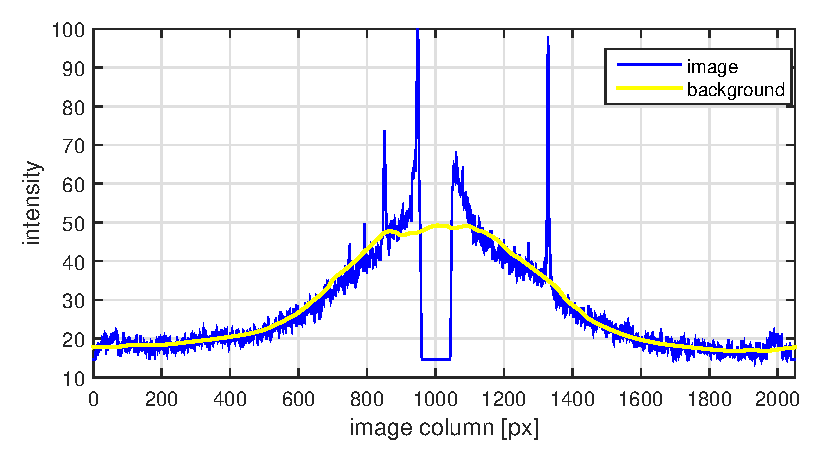
\includegraphics[width=.8\textwidth]{image_rust2.eps}
     \caption[Filtrace pozadí.]{Filtrace pozadí v HDR snímku znázorněná v řádku obrazu protínajícím obraz podstavce na kámen, který komplikuje odhad pozadí.}
        \label{fig:pozadi}
\end{figure}
	       

\subsection*{Určení vlastností laserových svazků}
Popis svazku může obsahovat tyto parametry: směr šíření svazku určený azimutem a elevací, velikost svazku, zářivý tok, intenzitu a směr světelných ocásků laserové stopy. Nově jsme si ukázali, že můžeme do popisu zahrnout velikost a směr posunu svazku při rotaci kamene. Popis svazku lze obohatit o dominantní orientaci, ke které můžeme přidat eliptický tvar stopy. 

Vlastnosti laserových svazků určíme z filtrovaného snímku, od kterého odečteme pozadí. Filtrace pozadí je znázorněna na obr. \ref{fig:pozadi}. MSER oblasti jsou roztříděny, podle toho, ke které stopě patří. Oblasti s nízkou prahovou hodnotu mohou náležet více než jedné stopě. Pro stopy   následně určíme následující parametry:

\begin{itemize}
	\item \textbf{Azimut a elevace} - Pozici světelné stopy v obraze lze určit jako polohu pixelu s maximální intenzitou v detekované oblasti. Šum v obraze ale situaci komplikuje a lepší odhad získáme, pokud určíme pozici stopy jako těžiště vrchní vrstvy pyramidy MSER oblastí příslušné stopy. Přesněji střed eliptické aproximace vrchní vrstvy. 
	
	Snímek ze zatížen radiálním zkreslením, které je způsobeno vlastností optické soustavy objektivu. Radiální zkreslení bylo určeno v předchozí bakalářské práci \cite{Drapela}, odkud navíc známe transformaci mezi pozicí bodu v nezkresleného snímku a odpovídajícím parametrům azimutu a elevace.
	
	\item \textbf{Velikost} - Pro všechny MSER oblasti určíme počet světelných stop, které se v dané oblasti nachází. Předpokládá se, že každé stopě náleží alespoň jedna MSER oblast, která obsahuje pouze tento samostatný svazek. Může ovšem nastat situace, že první vrstva pyramidy MSER oblastí, která obsahuje danou stopu, náleží také intenzivnější stopě. Méně intenzivní stopa je poté vyřazena a celá oblast přenechána významnější stopě. 
	
 	Určíme nejrozsáhlejší oblasti, které obsahují minimální počet stop a dále již počítáme pouze s nimi. U těch oblastí, které obsahují pouze jednu stopu určíme velikost a přiřadíme ji k daném svazku. Velikosti zbylých oblasti postupně dělíme podle poměru velikostí svazků před rozdělením, dokud takto nerozdělíme všechny oblasti.   
	\item \textbf{Zářivý tok} - Zářivý tok určíme obdobným postupem jako při výpočtu velikosti světelné stopy. Zářivý tok je zde součtem intenzit v dané oblasti po odečtení pozadí.   
	\item \textbf{Intenzita} - Intenzitu určíme výpočtem jako poměr zářivého toku a velikosti světelného svazku.
	\item \textbf{Orientace a eliptický tvar} -  Pro každou MSER oblast je určena elipsa, která uzavírá danou oblast. U této elipsy lze určit její orientaci. Stopa může obsahovat více MSER oblastí. Orientace stopy je určena jako medián orientací elips všech MSER oblastí a hlavní poloosy eliptického tvaru stopy jsou určeny podle MSER oblasti, která je prostřední vrstvou všech oblastí. Orientace a eliptický tvar mohou být zároveň úzce spjaty s orientací světelných ocásků.		
		
\end{itemize}

\section*{Světelné ocásky}
	V ideálním případě lze ve snímaném obraze pozorovat pouze dopady světelných svazků, které vznikly kombinací odrazů a lomů zdrojového svazku od faset broušeného kamene. U reálného kamene ovšem v obraze pozorujeme tenké slábnoucí přímky vycházející ze stopy světelného svazku (ocásky). Tyto ocásky vznikají díky lomu/odrazu světelného svazku od neostrých hran broušeného kamene. Hrany modelujeme v LADOKu jako posloupnost tenkých plošek s nenulovým poloměrem křivosti.
	
\begin{itemize}
	\item Při \textbf{odrazu} světelného svazku od hrany vzniknou v modelovém případě rovnoměrně rozmístěné svazky ležící ve stejné rovině jako svazky, které vznikly odrazem od faset propojených touto hranou.  	

	\item V případě \textbf{lomu} světelného svazku přes hranu kamene je koncentrace lomených svazků největší u svazku lomeného přes sousední fasetu kamene.  
\end{itemize}	  

\begin{figure}[h!]
\begin{center}
\scalebox{.9}{ \input{xfig/tails.pstex_t}}
\end{center}
\caption{Příklad snímaného obrazu s vyznačením svazků a ocásků.}
\label{fig:tail_ex1}
\end{figure}

	Se znalostí směru a velikosti ocásků detekovaných svazků dostáváme nové informace, které nohou přispět k jejich správnému párování se svazky z matematického modelu kamene.
	Ve snímaném obraze nelze rozpoznat všechny vznikající ocásky, ale pouze ty s dostatečně velkou intenzitou. Intenzita je přitom ovlivněna množstvím faktorů, jako je např. zářivý tok svazku, délka hrany, dopadající úhel, čistota hrany atd. Všechny faktory, které ovlivňují intenzitu ocásku prozatím nejsme schopni v programu LADOK zahrnout do matematického modelu, proto pro prování svazků bude užitečná především informace o směru ocásku. 
	
	
\section*{Detektor ocásků}
	Princip detektoru ocásků zjednodušeně spočívá v převodu okolí stopy do polárních souřadnic (vzdálenost $\rho$ a úhel $\phi$) a nalezení oblastí úhlů, ve kterých je patrný výrazný vzestup intenzity oproti okolí. Takovéto oblasti jsou typicky důsledkem přítomnosti ocásků o obraze a lze tímto způsobem ocásky detekovat. 
	
	 U rozvinutí do polárního grafu si však musíme všimnout překážek, které komplikují detekci ocásků.  
	 \begin{itemize}	 	
	 	\item V blízkém okolí jedné stopy se může nacházet další stopa. V polárním grafu se tato blízká stopa jeví jako ocásek a dochází k falešné detekci.	
	 	\item Stopy a ocásky jsou v obraze různě velké. Je třeba efektivně určovat vzdálenost $\rho$ do které budeme převádět okolí stopy do polárního grafu. Pokud zvolíme malé $\rho$ nepokryjeme oblast, kde se vyskytují ocásky a velké $\rho$ zvýší časovou náročnost výpočtu.   	
	\end{itemize}
	
	Elegantní řešení přináší použití MSER detektoru, pomocí něhož získáme vymezení oblasti a tím i vzdálenosti $\rho$, kde se stopa i s ocásky nachází. Se znalostí oblastí náležící jednotlivým stopám jsme schopni od sebe stopy částečně oddělit a redukovat množství falešných detekcí. Na druhou stranu sousední stopa muže ležet na pozici ocásku a odstraněním sousední stopy odstraníme současně i ocásek, který prozatím nejsme schopni v případě překrytí oddělit. Vzhledem k rozmanitosti stop, co do velikosti, intenzity, množství a tvaru ocásků apod. není jednoduché stopu matematicky modelovat. Pokud by se podařilo vytvořit dostatečně přesný kompaktní model stopy, je možné uvažovat o situaci, kdy budeme schopni od sebe separovat překrývající se stopy a ocásky. 
	
 Pro znázornění postupu a mezivýsledků jsme si vybrali laserovou stopu (obr.\ref{fig:mark_tail}), která v obraze nekoliduje s další výraznou stopu. Zvolená stopa vznikla dopadem laserového svazku typu ...!!doplnit(až budou popsány všechny třídy svazků)!!.... V obraze jsou patrné čtyři ocásky různě intenzity. 
	

	\begin{figure}[htp]
	\centering
	\begin{minipage}[c]{0.4\textwidth}
	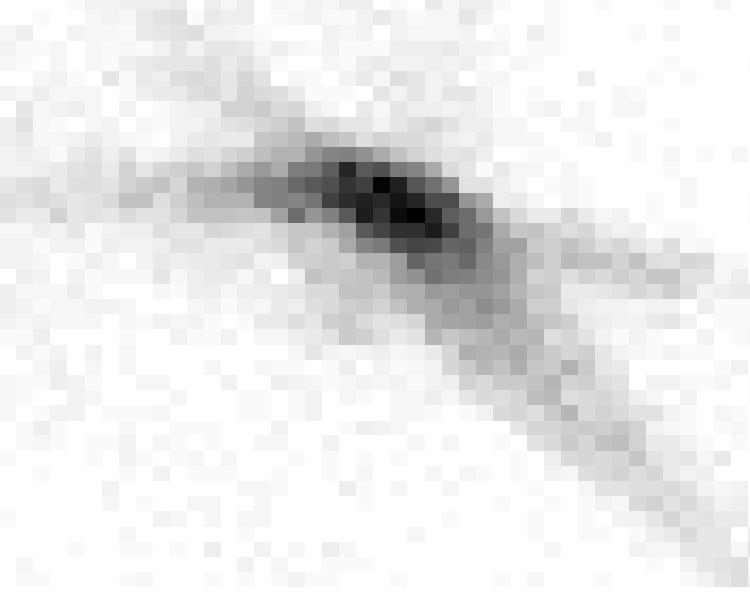
\includegraphics[width=\textwidth]{figures/tail07.pdf}
	\end{minipage}
	\begin{minipage}[c]{0.4\textwidth}
	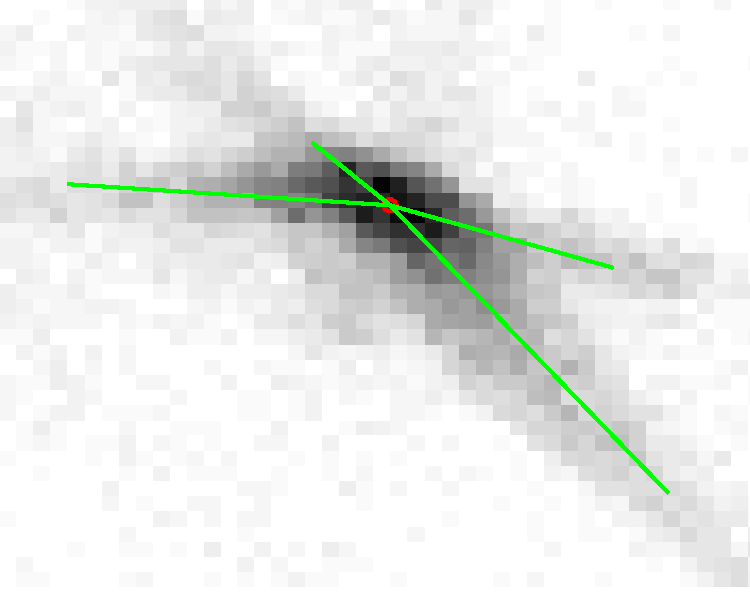
\includegraphics[width=\textwidth]{figures/tail08.pdf}
	\end{minipage}\\
	\begin{minipage}[c]{0.4\textwidth}
	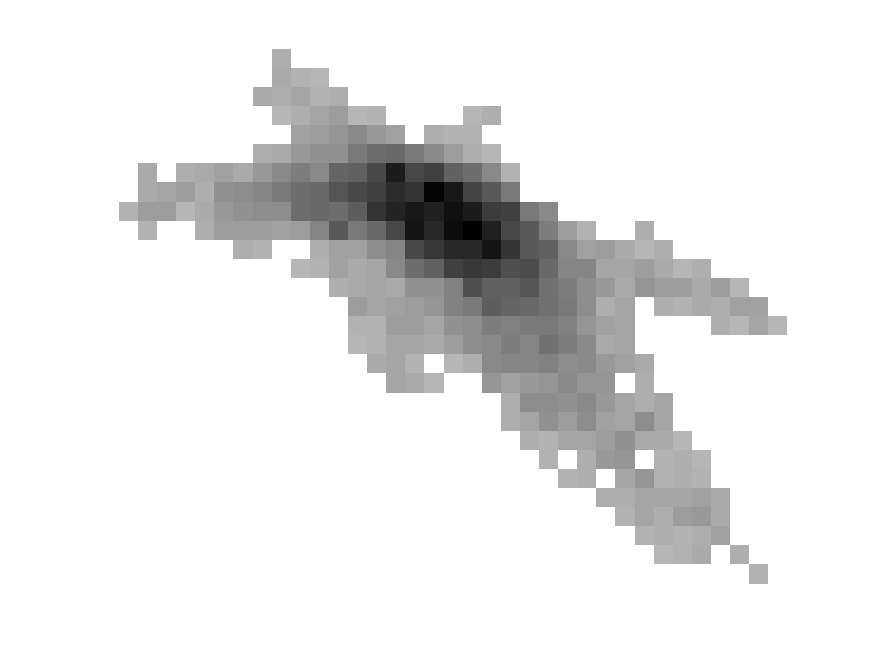
\includegraphics[width=\textwidth]{figures/tailex01.pdf}
	\end{minipage}
	\begin{minipage}[c]{0.4\textwidth}
	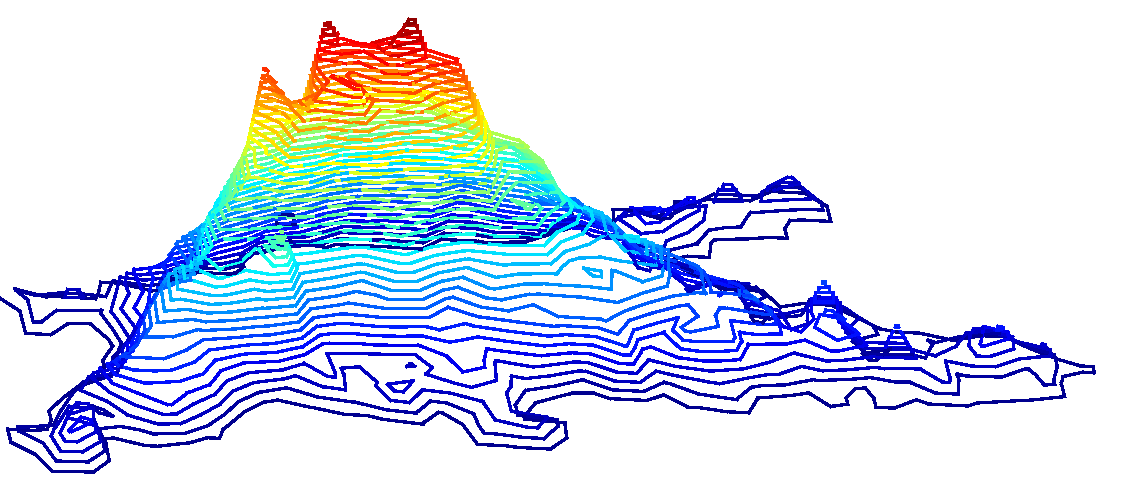
\includegraphics[width=\textwidth]{figures/tailex02.pdf}
	\end{minipage}
	
	\caption[Detektor ocásků - laserová stopa.]{Zvolená laserová stopa k ilustraci algoritmu detektoru ocásků. Stopa vznikla dopadem svazku typu $\dots \dots$ na stínítko. V měřicí soustavě byl přitom umístěn kámen typu \textit{VIVA $12$} s odstínem \textit{Crystal} a průměrem \SI{4.8}{\milli\meter}. Snímek vpravo nahoře znázorňuje výřez stopy ze snímaného obrazu. Můžeme zde pozorovat čtyři ocásky s různými vlastnostmi. Vlevo nahoře je výsledek detekce popsané níže. Obrázek vpravo dole ukazuje MSER oblast a poslední obrázek znázorňuje 3D pohled na zkoumanou stopu.}
	\label{fig:mark_tail}
	\end{figure}


Jednotlivé kroky algoritmu: 
	\begin{itemize}
	\item Vybereme stopu, u které chceme identifikovat ocásky a ze snímku vybereme oblast (obr.\ref{fig:mark_tail}), která náleží zkoumané stopě. 
	
	\item Po odečtení okolního šumu $z_{noise}$ prahujeme intenzitu pixelů stopy $2$krát střední hodnota intenzity $z_{mean}$. Pixely s intenzitou vyšší než zvolený práh nastavíme intenzitu odpovídající prahové hodnotě a posuneme $z_{noise}$ na hodnotu $z_{mean}$ tak, že ke všem pixelům přičteme intenzitu $z_{mean}$. Důvodem tohoto kroku je snaha odstranit nežádoucí vlastnosti velkého šumu v hodnotách intenzity v blízkém okolí "těžiště" stopy a také to, že se chceme zvětšit relativní příspěvek pixelů s nižší intenzitou do součtového kritéria \ref{eq:Isuma}.   
	
	\item Stopu s velikostí okolního šumu $z_{mean}$ převedeme do polárních souřadnic ($\rho$, $\phi$). Intenzitu $I_{pol}$ v polárním grafu $I_{pol} = f(\phi,\rho)$ určujeme pomocí bipolární interpolace, která pro větší efektivitu vynechává oblasti mimo oblast stopy, kde $I_{pol} = 0$. Důležitým parametrem při interpolaci je velikost vzorkování $f_{\phi}$ úhlu $\phi$ resp. vzorkování $f_{\rho}$ vzdálenosti $\rho$ . Experimentálně jsme zvolili $f_{\phi} = \SI{3}{\degree}$ a $f_{\rho} = \SI{1}{\px}$. Interpolaci počítáme v intervalech  $\phi \in \left\langle 0,2\pi \right\rangle$ a $\rho \in \left\langle 1,\rho_{max} \right\rangle$, kde $\phi_{max}$ je maximální vzdálenost všech pixelů v oblasti stopy od její pozice.  
	
	\begin{figure}[htbp]
    \centering
    \begin{minipage}[c]{0.48\textwidth}
        \centering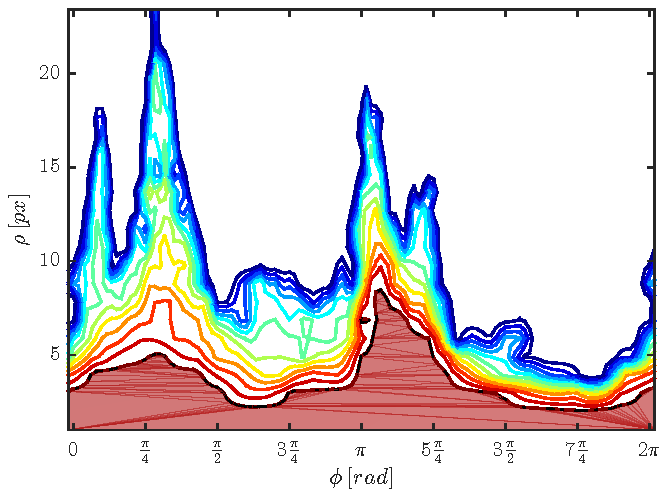
\includegraphics[width=.98\textwidth]{tailex03.pdf}
    \end{minipage}
    \begin{minipage}[c]{0.48\textwidth}
        \centering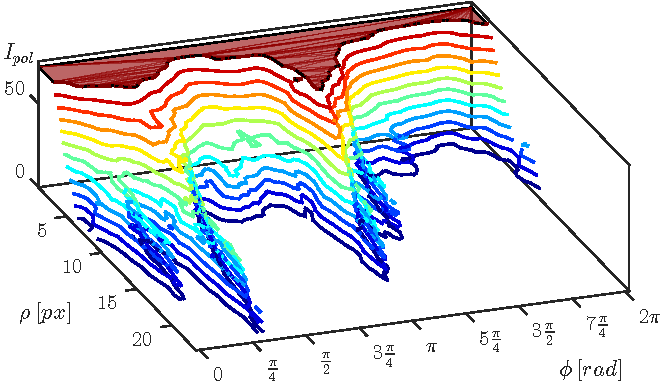
\includegraphics[width=.98\textwidth]{tailex04.pdf}
    \end{minipage}
    \\
        \caption[Detektor ocásků - polární graf.]{Dva pohledy na intenzitu okolí stopy převedené do polárního grafu $I_pol$ zobrazené pomocí vrstevnic.}
        \label{Detekce}
\end{figure}
	
	\item Provedeme součet intenzit $I_{pol}$ pro jednotlivé úhly $\phi$ od minimální do maximální vzdálenosti $\rho$ a získáme závislost $I_\phi = f(\phi)$, kde  
	
	\begin{equation}
	I_{\phi_i} = \sum_{j = 1}^{\rho_{max}} I_{pol}\left(i,j\right)\,. \hspace*{2cm} i \in \left\lbrace 0, \frac{3}{180}\pi, \dots \,,2\pi \right\rbrace
	\label{eq:Isuma}
	\end{equation}
	Následně na $I_{\phi}$ aplikujeme kubickou interpolaci sousedních hodnot s $5$krát citlivějším vzorkováním $f_{\phi_2} = \frac{f_{\phi}}{5}$ a rozšíříme rozsah $\phi$ na $\phi \in \left\langle -\frac{\pi}{2},\frac{5}{2}\pi \right\rangle$. 
	
	\item Graf závislosti $I_\phi = f(\phi)$ filtrujeme konvolucí s gausiánem $g(x)$ se směrodatnou odchylkou $\sigma = 3$ a získáme referenční závislost $I_{filt}$.
	
	\begin{equation}
		g(x) = \frac{1}{\sqrt{2\pi} \cdot \sigma}e^{-\frac{x^2}{2\sigma^2}}\,.
	\end{equation}
	
	\begin{figure}[htbp]
    \centering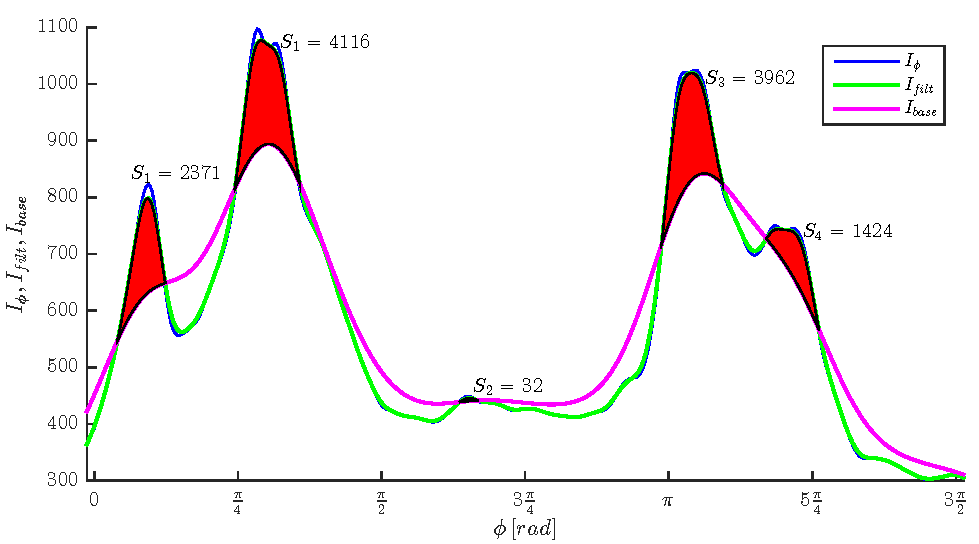
\includegraphics[width=\textwidth]{figures/tailex05.pdf}
     \caption[Detekce ocásků - zpracování polárního grafu.]{Grafické vysvětlení funkce algoritmu pro detekci ocásků. }
    \label{fig:tailSumGraph}
	\end{figure}
	
	\item Na graf $I_{filt}$ následně opakovaně aplikujeme konvoluci, tentokrát s gausiánem $g(x)$ s vyšší směrodatnou odchylkou $\sigma = 8$, abychom získali základnu $I_{base}$, kterou budeme porovnávat se signálem $I_{filt}$.
	
	\item Nalezneme souvislé oblasti $\mathcal{R}_1, \dots , \mathcal{R}_n$, kde graf $I_{filt}$ má větší hodnotu než $I_{base}$ a sečteme rozdíly $I_{filt}$ a $I_{base}$ v jednotlivých vzorcích. Velikost součtu $S_1, \dots , S_n$ závisí na vzorkovací frekvenci $f_{\phi_2}$.
	
	\begin{equation}
	S_i = \sum_{\phi_j \colon \phi_j \in \mathcal{R}_i}I_{filt}(\phi_j)-I_{base}(\phi_j)\,. \hspace*{2cm} i \in \left\lbrace 1, 2, \dots \,, n \right\rbrace
	\label{eq:Rsuma}
	\end{equation}
	
	\item Za ocásek uvažujeme oblast $\mathcal{R}_i$, kde je součet $S_i$ větší než prahovací úroveň $s_{th}$ (pro $f_{\phi_2}$ je $s_{th} = 500$). Směr ocásku $\varphi$ je určen jako úhel, ve kterém je graf $I_{filt}$ v dané oblasti maximální a velikost ocásku $\varrho_i$ určuje $\rho_{max}$ a poměr součtu $S_i$ k maximálnímu v pro danou stopu.  
	
	\begin{equation}
	\varphi_i = \argmax_{\phi_j \colon \phi_j \in \mathcal{R}_i}I_{filt}(\phi_j) \,, \hspace{1cm} \varrho_i = \frac{S_i}{\max_{j \in 1,\dots , n}S_j}\rho_{max}\,.
	\label{eq:tail_params}
	\end{equation}
		
	\begin{figure}[htbp]
    \centering
    \begin{minipage}[c]{0.48\textwidth}
        \centering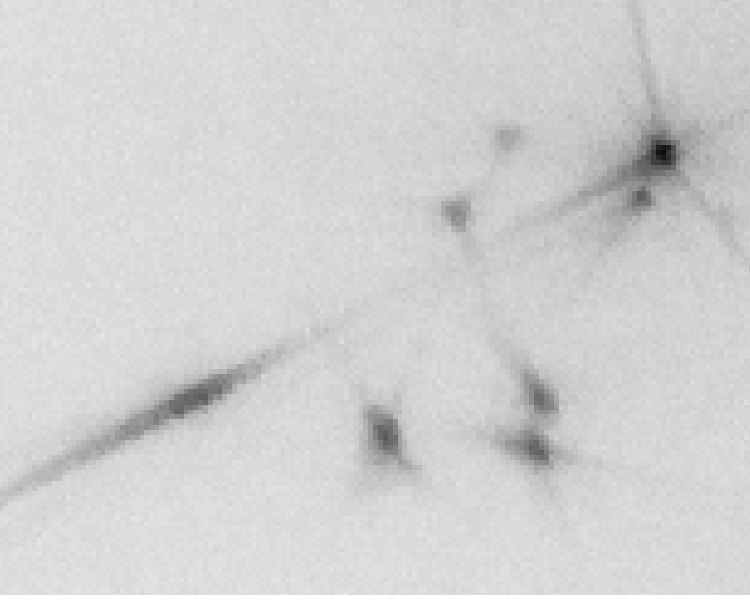
\includegraphics[width=.98\textwidth]{tail01.pdf}
    \end{minipage}
    \begin{minipage}[c]{0.48\textwidth}
        \centering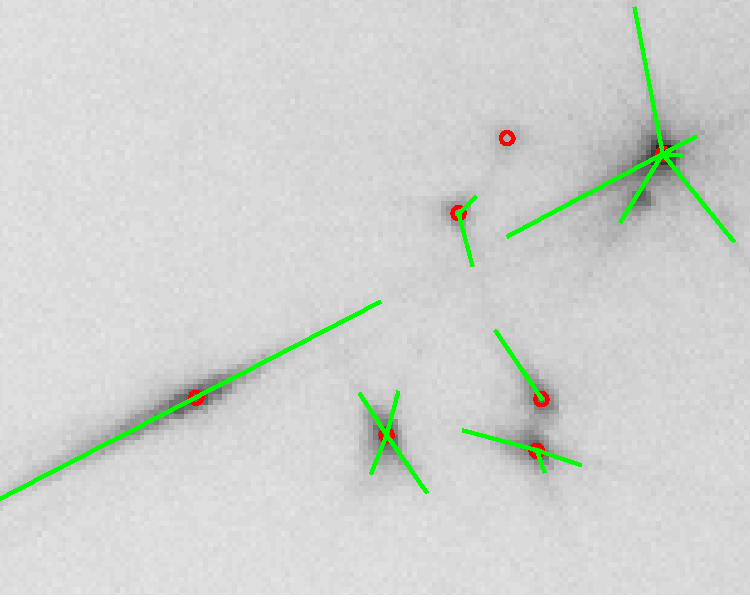
\includegraphics[width=.98\textwidth]{tail02.pdf}
    \end{minipage}
    \\
        \caption[Detektor ocásků - příklad detekce.]{Ukázka funkce detektoru ocásků na vybraném vzorku z obrazu. }
        \label{Detekce}
\end{figure}


	
	
\end{itemize}	   
	
	

\section{MSER detector configuration parameter list}	
	Here is a list of the configuration parameters used for beam detection setting. All of them can be used with their default values. This description of the parameters can be usefull for understanding the algorithm or debugging.
	
\begin{center}


\begin{tabular}{l|l|p{8cm}}
    \textbf{Name} 		& \textbf{Default} & \textbf{Description} \\ \hline \hline 
    \textit{BackgroundFilt}	    	& $201$ 	& Size of Gaussian filter mask used for background estimation. \textit{Sigma} of mask is equal to \textit{BackgroundFilt} \\ \hline
    \textit{BackgroundKMean}    	& $0.15$	& $BackgroundKMean \times mean(image)$ is added to background estimation. \\ \hline
    \textit{ComputeAllLayers}   	& $1$		& $1$ - Divide all layers in marks variable calculation. $0$ - Calculate only with upper layers. \\ \hline
    \textit{ComputeTails}   		& $ 1 $		& $1$ - Tails of marks are computed. It takes some time. $0$ - No tails. Faster.\\ \hline    
    \textit{CleanerAxisRatio}   	& $ 10 $	& MSER regions with upper axis ratio are deleted. \\ \hline
    \textit{CleanerFilterSigma}  	& $ 5 $		& \textit{Sigma} of filter mask in image blurring. \\ \hline
    \textit{CleanerFilterSize}   	& $ 31 $	& Size of filter mask in image blurring.\\ \hline
	\textit{CleanerMean}    		& $ 0.035 $ & Regions with peak where difference of mean of surrounding
intensity is lower than $CleanerMean \times mean(image)$ are deleted. \\ \hline
    \textit{CleanerSumWide} 		& $ 5 $		& Size of surrounding in cleaning process.  \\ \hline
    \textit{FilterSigma}    		& $ 0.7 $	& \textit{Sigma} of niose reducing filter mask. \\ \hline
    \textit{FilterSize} 			& $ 3 $		& \textit{Size} of niose reducing filter mask.\\ \hline 
    \textit{MSERMaxAreaVar} 		& $ 0.9 $	& This value specifies the step size between intensity threshold levels used in selecting extremal regions while testing for their stability. Decrease this value to return more regions.\\ \hline
    \textit{MSERRegion} 			&$[2\,,\, 14000]$& Two-element vector, [minArea maxArea], which specifies the size of the regions in pixels. This value allows the selection of regions containing pixels between minArea and maxArea, inclusive.\\ \hline
    \textit{MSERThresh} 			& $ 1.2 $	& Increase this value to return a greater number of regions at the cost of their stability. Stable regions are very similar in size over varying intensity thresholds.\\ \hline
    \textit{SurroundThres}   		& $ 0.8 $	& Multiple of $mean(image)$ where surrounding intensity is moved.   \\ 
\end{tabular}

\end{center}

%\clearpage